%%
%% This is file `sample-manuscript.tex',
%% generated with the docstrip utility.
%%
%% The original source files were:
%%
%% samples.dtx  (with options: `manuscript')
%% 
%% IMPORTANT NOTICE:
%% 
%% For the copyright see the source file.
%% 
%% Any modified versions of this file must be renamed
%% with new filenames distinct from sample-manuscript.tex.
%% 
%% For distribution of the original source see the terms
%% for copying and modification in the file samples.dtx.
%% 
%% This generated file may be distributed as long as the
%% original source files, as listed above, are part of the
%% same distribution. (The sources need not necessarily be
%% in the same archive or directory.)
%%
%% The first command in your LaTeX source must be the \documentclass command.
\documentclass[manuscript]{acmart}

%% Remove ACM Reference Format line for arXiv copy
%\settopmatter{printacmref=false}




%TODO: My statement that a straight line in a log-log plot gives a polynomial relationship has to be false, because a straight line in a linear plot becomes a curve in a log-log plot.

%TODO: From brucifer on reddit: I'm only about 1/3 of the way through right now, but one minor correction: Ford doesn't actually mention PEGs in his 2002 thesis about packrat parsers, they're not introduced until his 2004 paper on PEGs. There's also related work dating back to the '60s and '70s. (Ford cites this paper from '70: https://bford.info/packrat/ref/birman70tmg.pdf and this one from '73: https://core.ac.uk/download/pdf/82258594.pdf )


%TODO: Aaron Moss gave great feedback on the pika parser, send him the squirrel parser paper too: "Fascinating work, I’m always interested to see a new PEG parsing algorithm, and handling left-recursion as cleanly as you did is impressive."...






%% Even left/right margins for arXiv copy
\evensidemargin 0.25in
\oddsidemargin 0.25in

%% Rights management information.  This information is sent to you
%% when you complete the rights form.  These commands have SAMPLE
%% values in them; it is your responsibility as an author to replace
%% the commands and values with those provided to you when you
%% complete the rights form.
\setcopyright{acmlicensed}
\copyrightyear{2025}
\acmYear{2025}
\acmDOI{00.0000/0000000.0000000}

%%
%% These commands are for a JOURNAL article.
\acmJournal{TOPLAS}
\acmVolume{0}
\acmNumber{0}
\acmArticle{0}
\acmMonth{8}

%%
%% Submission ID.
%% Use this when submitting an article to a sponsored event. You'll
%% receive a unique submission ID from the organizers
%% of the event, and this ID should be used as the parameter to this command.
%%\acmSubmissionID{123-A56-BU3}

%%
%% The majority of ACM publications use numbered citations and
%% references.  The command \citepstyle{authoryear} switches to the
%% "author year" style.
%%
%% If you are preparing content for an event
%% sponsored by ACM SIGGRAPH, you must use the "author year" style of
%% citations and references.
%% Uncommenting
%% the next command will enable that style.
%%\citepstyle{acmauthoryear}

\usepackage[utf8]{inputenc}
\usepackage[english]{babel}

\usepackage{hyperref}
\hypersetup{
    colorlinks=true,
}

\usepackage[newfloat]{minted}
\usemintedstyle{algol_nu}
\setminted[dart]{
frame=lines,
framesep=2mm,
baselinestretch=1.2,
fontsize=\footnotesize,
linenos,
xleftmargin=4mm,
numbersep=2mm,
breaklines
}

\usepackage{caption}
\usepackage{subcaption}

% https://tex.stackexchange.com/questions/254044/caption-and-label-on-minted-code
\newenvironment{code}{\captionsetup{type=listing}}{}
\SetupFloatingEnvironment{listing}{name=Listing}

% Prevent footnote page breaks
\usepackage{manyfoot}

\usepackage{bm}

\newtheorem{theorem}{Theorem}
\newtheorem{coroll}{Corollary}
\newtheorem{defn}{Definition}
\newtheorem{lemma}[theorem]{Lemma}

\newfloat{grammar}{h}{Grammar}

\usepackage{graphicx}

% Needed for \toprule
\usepackage{booktabs}

%%
%% end of the preamble, start of the body of the document source.
\begin{document}

%%
%% The "title" command has an optional parameter,
%% allowing the author to define a "short title" to be used in page headers.
\title[The Squirrel Parser]{The squirrel parser: a packrat parser capable of left recursion}

%%
%% The "author" command and its associated commands are used to define
%% the authors and their affiliations.
%% Of note is the shared affiliation of the first two authors, and the
%% "authornote" and "authornotemark" commands
%% used to denote shared contribution to the research.
\author{Luke A. D. Hutchison}
\email{luke.hutch@alum.mit.edu}
\orcid{0000-0002-2937-8619}
%\affiliation{\institution{Massachusetts Institute of Technology}}

%%
%% By default, the full list of authors will be used in the page
%% headers. Often, this list is too long, and will overlap
%% other information printed in the page headers. This command allows
%% the author to define a more concise list
%% of authors' names for this purpose.
% \renewcommand{\shortauthors}{Luke A. D. Hutchison}

%%
%% The abstract is a short summary of the work to be presented in the
%% article.
\begin{abstract}
The \emph{squirrel parsing algorithm} provides a simple, elegant, and universal solution to the decades-old problem of left-recursive cycles in recursive descent parsing. Recursive descent parsers, including memoizing packrat parsers, have not previously supported left recursive grammars without special care, because any cycle in the grammar that consumes zero input characters triggers infinite recursion. Numerous mechanisms have been proposed for handling left recursion, including rewriting the grammar into non-left-recursive form (which affects the structure of the resulting parse tree), and a variety of other complex parser modifications. This paper carefully re-examines the problem of left recursion, culminating in the design of the squirrel parser, a surprisingly simple modification of the packrat parser to directly support all forms of left recursion in a single unified way, including direct, indirect, input-dependent, and interwoven left recursive cycles, to any degree of complexity. The worst-case time and space complexity of squirrel parsing remains linear in the length of the input, incurring virtually no extra time or space overhead compared to packrat parsing without left-recursive grammar rules, which means that the squirrel parser operates close to the theoretical maximum speed for a memoizing recursive descent parser, while handling grammars of any structure or complexity.
\end{abstract}

%%
%% The code below is generated by the tool at http://dl.acm.org/ccs.cfm.
%% Please copy and paste the code instead of the example below.
%%
\begin{CCSXML}
<ccs2012>
   <concept>
       <concept_id>10011007.10011006.10011041.10011688</concept_id>
       <concept_desc>Software and its engineering~Parsers</concept_desc>
       <concept_significance>500</concept_significance>
   </concept>
   <concept>
       <concept_id>10003752.10003766.10003771</concept_id>
       <concept_desc>Theory of computation~Grammars and context-free languages</concept_desc>
       <concept_significance>400</concept_significance>
   </concept>
 </ccs2012>
\end{CCSXML}

\ccsdesc[500]{Software and its engineering~Parsers}
\ccsdesc[400]{Theory of computation~Grammars and context-free languages}

%%
%% Keywords. The author(s) should pick words that accurately describe
%% the work being presented. Separate the keywords with commas.
\keywords{parsing, recursive descent parsing, top-down parsing, PEG parsing, PEG grammars, packrat parsing, precedence, associativity, left-recursive grammars, left recursion, memoization}

%%
%% This command processes the author and affiliation and title
%% information and builds the first part of the formatted document.
\maketitle

\section{Introduction}

%TODO: add PEG parsing rule info in intro
%TODO: note that without OneOrMore (or equivalently, the ability to form grammar cycles in conjunction with Seq, which is the recursive equivalent of OneOrMore), PEG would be strictly less powerful.

% Explain packrat parsing, and PEG

\subsection{\label{sec:rec_desc}Recursive descent parsing}

The earliest described parsing algorithms, used to parse programs written in ALGOL60~\cite{irons1961syntax,lucas1961structure}, were recursive algorithms that primarily worked top-down. Despite many developments in parsing algorithms since those early days~\cite{kegler2023parsing}, recursive descent parsing has remained popular, because it is simple to implement, and because the structure of a recursive descent parser's code directly mirrors the structure of the underlying grammar. However, recursive descent parsers have suffered from three significant drawbacks: (1) in their early formulations, they were inefficient, because they needlessly repeated work; (2) they could not handle left-recursive grammars without entering an infinite loop; and (3) it was difficult to implement a recursive descent parser that could robustly recover from a syntax error. % TODO: talk about error recovery?

% TODO: parallel these three below, and pull citations from the PikaParser paper

It was discovered that memoization could significantly improve the performance of recursive descent parsing~\cite{norvig1991}, even to the point that recursive descent parsers could run in time linearly proportional to the length of the input using a technique known as ``packrat parsing'', proposed by Ford in his 2002 Master's thesis~\cite{ford2002}. Along with that innovation, the Parsing Expression Grammars (PEG) formalism was also born as a new and simple way to specify recursive descent grammars~\cite{ford2002,ford2002b,ford2004}.

\subsection{\label{sec:peg_grammars}Parsing Expression Grammars (PEG)}

In contrast to the parsing algorithms and grammar formalisms at the time, which presented grammar rules as generative productions or derivations, PEG rules represented \emph{greedily-recognized patterns,} replacing ambiguity with deterministic choice (PEG grammars are unambiguous for any given input). All PEG rules can be implemented in a straightforward way (Table~\ref{tab:peg_operators}): given the current parsing position, each non-terminal grammar clause determines whether or not it matches a subsequence of the input given whether or not its subclauses match a subsequence of the input, and when a match is found, the parsing position advances by the length of the match.

There are only four main PEG clause types: \texttt{Seq} advances the parser forwards through a series of subclause matches; \texttt{First} (ordered choice) matches as soon as one of its subclauses (tried in order) is found to match; \texttt{OneOrMore} matches a sequence of at least one instances of its subclause; and \texttt{NotFollowedBy} is a lookahead operator that does not consume any of the input, but matches if its subclause does not match at the current position. There are three more PEG clause types that can either be implemented directly or derived from the first four: \texttt{Optional} matches zero or one instances of its subclause; \texttt{ZeroOrMore} matches zero or more instances of its subclause; and \texttt{FollowedBy} is a lookahead operator that only matches if its subclause matches at the current position, but does not consume any of the input matched by its subclause. Each subclause $e_i$ can be either another grammar clause, or a terminal that matches zero or more characters of the input.

\begin{table*}[tbp]
    \centering
    {\small
    \begin{minipage}{0.45\textwidth}
        \centering
        \begin{tabular}{lcc}\toprule
        \textbf{Name}          & \textbf{Num subclauses} & \textbf{Notation}     \\\midrule
        \texttt{Seq}           & 2+                      & $e_1$ $e_2$ $e_3$     \\
        \texttt{First}         & 2+                      & $e_1$ / $e_2$ / $e_3$ \\
        \texttt{OneOrMore}     & 1                       & $e+$                  \\
        \texttt{NotFollowedBy} & 1                       & $!e$                  \\\bottomrule
        \end{tabular}
        \subcaption{Principal PEG operators}
        \label{tab:peg_standard}
    \end{minipage}
    \hfill
    \begin{minipage}{0.45\textwidth}
        \centering
        \begin{tabular}{lcc}\toprule
        \textbf{Name}       & \textbf{Notation} & \textbf{Equivalent to} \\\midrule
        \texttt{Optional}   & $e?$              & $e / \epsilon$         \\
        \texttt{ZeroOrMore} & $e*$              & ${e+} / \epsilon$      \\
        \texttt{FollowedBy} & $\&e$             & $!!e$                  \\\bottomrule
        \end{tabular}
        \subcaption{Derived PEG operators}
        \label{tab:peg_derived}
    \end{minipage}
    }
    \caption{\label{tab:peg_operators}PEG operators, defined in terms of subclauses $e$ and $e_i$, and the empty string $\epsilon$.}
    \Description[PEG operators]{PEG operators split into standard and derived operators, defined in terms of subclauses $e$ and $e_i$, and the empty string $\epsilon$.}
\end{table*}

As a subset of all possible recursive rule types, all non-left-recursive PEG grammars can be parsed directly by a recursive descent parser, and can be parsed efficiently with a packrat parser. PEG grammars are more powerful than regular expressions, but it is conjectured (though as yet unproved) that there exist context-free languages that cannot be recognized by a PEG parser~\citep{ford2004}). PEG parsers suffer from the same limitations as other recursive descent parsers: they cannot parse left-recursive grammars without special handling, and they have poor error recovery properties.

A PEG grammar consists of a finite set of \emph{rules}. Each rule has the form $A \leftarrow e$, where $A$ is a unique \emph{rule name}, and $e$ is a \emph{parsing expression}, also referred to as a \emph{clause}. One rule is designated as the \emph{starting rule}, which becomes the root for top-down recursive parsing. PEG clauses are constructed from \emph{subclauses}, \emph{terminals}, and \emph{rule references}. The subclauses within a rule's clause may be composed into a tree, with \emph{PEG operators} forming the non-leaf nodes, and terminals or rule references forming the leaf nodes.

Terminals can match individual characters, strings, or (in a more complex parser) even regular expressions. One special type of terminal is the \emph{empty string} $\epsilon$ (with ASCII notation \texttt{()}), which always matches at any position, even beyond the end of the input string, and consumes zero characters.



Left recursion has confounded parser builders and grammar writers since the rise in popularity of top-down parsing algorithms two decades ago. Several attempts have been made to support left recursion when parsing, including recommendations on how to manually rewrite grammar rules into non-left recursive form, automatic rule rewriting into non-left-recursive form as a preprocessing step before parsing, and modifications to parsing algorithms to enable left-recursive grammars. Rule rewriting is far from ideal, because the semantic structure of the grammar is no longer directly represented in the structure of the parse tree, and because postprocessing of some form is needed to interpret the modified parse tree structure is if it were in semantically-representative form. Previous parser modifications to support unmodified left recursive grammars in the parser have resulted in complex parsing algorithms. A simple mechanism for directly supporting left recursion has previously resisted discovery.
%TODO: refs -- take language and refs from pika paper

\section{Deconstructing left recursion}

There are two reasons why left recursion is problematic in a recursive descent parser:



Left recursion cannot be interpreted as anything other than infinite recursion, unless we modify the definition of left recursion to require that every loop around a left-recursive cycle make nonzero progress towards the end of the input, because doing so ensures that the depth of recursion is bounded as a linear function of the length of the (finite) input. In other words, for parse tree nodes corresponding to positive matches of a left-recursive rule, each successively higher node in the parse tree must consume or match at least one additional character of the input.

In a memoizing parser, recursive frames cannot be memoized until they return. 

\begin{lemma}
Requiring each loop around a left recursive cycle to consume at least one additional character of the input ensures that recursive descent through a left recursive rule will eventually terminate with a mismatch (termed the \emph{fixed point} of the cycle). 
\end{lemma}

If any loop around a left recursive cycle were to consume zero characters, then recursive descent parsing would try to match the same rule at the same start position more than once in the same recursion path, resulting in a repeat of the ``parsing state'' or recursion parameters \texttt{(rule, pos)}, and therefore infinite recursion.

In recursive descent parsing, any higher recursion frame must match monotonically more characters than a lower recursion frame in the same recursive path. The length of the input is finite; therefore, in the extreme case, the topmost recursion frame for a left recursive rule may match the entire input. Each successively lower recursion frame must match at least one character fewer than the next-highest frame. Therefore, after a finite number of successively deeper recursion frames, left recursion must terminate with the rule matching fewer than zero characters of the input, i.e. no longer matching the input. We term this bottom-most mismatch of the left recursive rule \emph{the fixed point of the cycle}.

\begin{lemma}
A left recursive cycle should be matched against the input bottom-up, starting from the fixed point.
\end{lemma}

It is a common misconception that a recursive descent parser builds the parse tree from top to bottom. In reality, recursive descent parsing is a \emph{postorder} traversal of the grammar graph with respect to the input. A grammar clause is only determined to match the input after all required subclauses have been found to match the input. The corresponding parse tree node for a matching grammar clause is only created on exit from the corresponding recursion frame.

Therefore, in fact both top-down and bottom-up parsers build the parse tree from bottom to top. This makes intuitive sense, because the larger-scale structure of the input cannot be known until the finer-grained structure of the input has been determined.

This is sufficient reason to suspect that left recursion handling should also work from bottom to top. But there is a stronger reason to require it: it is not possible to know \emph{a priori} how many times to recurse into a left recursive loop (top-down) before terminating recursion at the fixed point. It is only possible to determine how many times a left-recursive cycle was able to match the input once it is not possible to find a longer match, which is a process of postorder traversal of the grammar with respect to the input. Also, it is only known \emph{a priori} that each loop around a left recursive cycle must consume at least one additional character of the input. However, it is not know exactly how many characters more than one should be consumed by a given loop around the cycle, until the number of characters consumed by the next-lowest loop around the cycle is known.

\begin{lemma}
Upwards expansion of a left recursive cycle should terminate when a successively longer match of the cycle can no longer be found.
\end{lemma}

Upwards expansion of a left recursive grammar cycle terminates when the condition that each loop around the cycle consume at least one additional character can no longer be satisfied.

In general, the intent of the grammar writer is probably for the parser to accept the longest possible match of a given left recursive grammar rule at a given start position, as opposed to accepting the mismatch resulting from an attempt to find an even longer match beyond that point. However, never allowing a match to become a mismatch may make certain grammars unparseable. %TODO: ref section here

% TODO: add fourth lemma, describing the need for cycle depth -- that a match of a loop around a grammar cycle will only ever incorporate a match from the previous loop around the same grammar cycle at the same position (and never from more than one loop previous).

\subsection{Algorithm sketch}

Given the lemmas presented above, we can arrive at a basic outline of an algorithm for handling left recursion in a recursive descent parser:

\begin{itemize}
    \item When entering a recursion frame to match a rule at a given input position, determine whether or not the parsing state \texttt{(rule, pos)} was visited in a higher frame of the current recursion path.
    \begin{itemize}
        \item If not, proceed with standard memoized recursive descent (packrat parsing) as normal.
        \item Otherwise, this is the fixed point of a left recursive cycle.
        \begin{itemize}
            \item Treat the current recursion frame as the fixed point of the cycle, resulting in a mismatch.
            \item Signal to the ancestral recursion frame with the same parsing state \texttt{(rule, pos)} that it needs to begin to iteratively expand the left recursive cycle upwards
        \end{itemize}
    \end{itemize}
    \item If the current recursion frame was marked for expansion of left recursion, iteratively keep trying to match the same rule at the same position until the match no longer increases in length (or becomes a mismatch).
    \item Only update the memo table for a rule if a match increases in length (and does not become a mismatch).
\end{itemize}

\begin{listing}[!ht]
\begin{minted}{dart}
MatchResult match(Clause clause, int pos) {
  var memoEntry = _memoTable.putIfAbsent(clause, () => LinkedHashMap()).putIfAbsent(pos, _MemoEntry.new);
  if (memoEntry.matchResult != null &&
      (memoEntry.inRecPath || memoEntry.memoVersion == this._memoVersionForPos[pos])) {
    return memoEntry.matchResult!;
  } else if (memoEntry.inRecPath) {
    memoEntry.foundLeftRec = true;
    memoEntry.matchResult = Mismatch.instance;
    return memoEntry.matchResult!;
  }
  memoEntry.inRecPath = true;
  do {
    final newMatchResult = clause.match(this, pos);
    if (memoEntry.matchResult != null && newMatchResult.len <= memoEntry.matchResult!.len) {
      break;
    }
    memoEntry.matchResult = newMatchResult;
    if (!memoEntry.foundLeftRec) {
      break;
    }
    memoEntry.memoVersion = ++this._memoVersionForPos[pos];
  } while (true);
  memoEntry.inRecPath = false;
  memoEntry.memoVersion = this._memoVersionForPos[pos];
  return memoEntry.matchResult!;
}
\end{minted}
\caption{The squirrel parser algorithm}
\label{listing:2}
\end{listing}


%TODO: Show a figure of this process

The ideas behind the upwards expansion of a left recursive cycle are, at the core, equivalent to those of Medeiros et al. and Warth et al.(?) %TODO: cite -- also the Mouse paper?
. However, the actual implementations of previous algorithms were complex, inefficient and unwieldy to reimplement. Furthermore, many existing algorithms for dealing with left recursion were only capable of dealing with \emph{direct} left recursion (where a rule refers to itself directly), and not indirect left recursion (where the path length of the left recursive cycle is greater than 1). % TODO: mouse, for example

It is possible to produce a much simpler and more efficient formulation of this left recursion expansion mechanism. We term this algorithm the \emph{squirrel parser}, in deference to the earlier packrat parser that also memoizes its match attempts. This new squirrel parsing algorithm is highly consise, simple, and extremely efficient, and it handles both direct and indirect recursion equally.

\section{Implementation of the squirrel parser}

Fig.~\ref{fig:Code} gives pseudocode for the squirrel parsing algorithm (lefthand side), and for several PEG clause types (righthand side).

\subsection{Pseudocode style}

The pseudocode style of Fig.~\ref{fig:Code} was chosen to be unambiguous, but generically understandable to anyone who has familiarity with C++, Java, C\#, D, or other C-like object oriented language. (This is preferable from an implementational point of view to the common practice of inventing a new human-level pseudocode for each new paper.)

Classes are designated with the toplevel keyword `\texttt{class}', followed by the class name, followed by an optional parenthesized list of parameters that represent fields within the class that are set by an implicit constructor. An abstract class may have abstract methods, which specify the method's parameter types and return type, but do not define a method body. The superclass of a class (here only \texttt{Clause}) optionally follows a class declaration, after a colon, and before the class body. Method and field/variable declarations follow the same general pattern as all C-like languages. Memory allocations (using the `\texttt{new}' keyword) cause all values to be initialized to zero, which effectively stores a zero, \texttt{null}, or \texttt{false} default value in fields or array elements at creation time. Local variables are declared with the keyword `\texttt{var}'. For-loops follow the standard C syntax. We use the shorthand notation \texttt{[]} for the empty array, and the notation \texttt{[m]} as shorthand for allocating an array consisting of a single element, \texttt{m}. Standard C pre-increment (\texttt{++x}) syntax is used for incrementing and then reading a value. The keyword `\texttt{const}' is used for an unmodifiable constant value.

\subsection{Pseudocode simplifications}

A couple of implementation details were omitted for brevity:

\begin{itemize}
    \item The \texttt{MemoTable} class (not shown) has just one method, \texttt{MemoEntry getOrCreate(Clause rule, int pos)}, which checks to see if there is already an entry in the memo table, indexed by the tuple \texttt{(rule, pos)}, and if not, creates a new (blank/zeroed-out) \texttt{MemoEntry} object, and stores it at position \texttt{(rule, pos)} in the memo table. Then either the existing or the newly-created \texttt{MemoEntry} instance is returned. \texttt{MemoTable} may be implemented either as a dense 2D array, for speed (at greater memory overhead), indexed by \texttt{rule} in the rows and \texttt{pos} in the columns, or as a sparse hashmap, to reduce memory consumption (incurring up to 2x performance penalty), keyed by the tuple \texttt{(rule, pos)}.

    \item Only about half of the PEG clause types are shown. The remainder are very straightforward to implement, following the pattern shown -- or the reference implementation of this parser can be consulted for a complete implementation. %TODO: ref
\end{itemize}

\begin{figure}
\centering
\begin{subfigure}[t]{.4\linewidth}
\begin{lstlisting}[frame=none,xleftmargin=-0.1\textwidth]
class Match(Clause clause, int pos, int len,
. . . . . . Match[] subClauseMatches);


const Match MISMATCH = new Match(null, -1, -1, []);


class Parser(Clause topRule) {
. String input;
. MemoTable memoTable;
. int[] cycleDepthForPos;
.
. Match match(Clause rule, int pos]) {
. . var memoEntry = memoTable.getOrCreateEntry(rule, pos);
. . return memoEntry.match(this, rule, pos);
. }
.
. Match parse(String inputStr) {
. . input = inputStr;
. . cycleDepthForPos = new int[input.length + 1];
. . memoTable = new MemoTable();
. . return match(topRule, 0);
. }
}


class MemoEntry {
. Match match;
. boolean inRecPath;
. boolean inLeftRecCycle;
. int cycleDepth;
.
. Match match(Parser parser, Clause rule, int pos) {
. . if (match == null
. . . . || cycleDepth < parser.cycleDepthForPos[pos]) {
. . . if (inRecPath) {
. . . . if (match == null) {
. . . . . inLeftRecCycle = true;
. . . . . match = MISMATCH;
. . . . }
. . . } else {
. . . . inRecPath = true;
. . . . while (true) {
. . . . . var newMatch = rule.match(parser, pos);
. . . . . if (match != null && newMatch.len <= match.len)
. . . . . . break;
. . . . . match = newMatch;
. . . . . if (!inLeftRecCycle)
. . . . . . break;
. . . . . cycleDepth = ++(parser.cycleDepthForPos[pos]);
. . . . }
. . . . inRecPath = false;
. . . }
. . . cycleDepth = parser.cycleDepthForPos[pos];
. . }
. . return match;
. }
}
\end{lstlisting}
\end{subfigure}
\hspace{5mm}
\begin{subfigure}[t]{.4\linewidth}
\begin{lstlisting}[firstnumber=59,frame=none,xleftmargin=.18\textwidth]
abstract class Clause {
. abstract Match match(Parser parser, int pos);
}


class First(Clause[] subClauses) : Clause {
. Match match(Parser parser, int pos) {
. . for (var i = 0;
. . . .  i < subClauses.length; i++) {
. . . var m = subClauses[i].match(parser, pos);
. . . if (m != MISMATCH) {
. . . . return new Match(this, pos, m.len, [m]);
. . . }
. . }
. . return MISMATCH;
. }
}


class Seq(Clause[] subClauses) : Clause {
. Match match(Parser parser, int pos) {
. . var ma = new Match[subClauses.length];
. . var p = pos;
. . for (var i = 0;
. . . .  i < subClauses.length; i++) {
. . . var m = subClauses[i].match(parser, p);
. . . if (m == MISMATCH) {
. . . . return MISMATCH;
. . . }
. . . ma[i] = m;
. . . p += m.len;
. . }
. . return new Match(this, pos, p - pos, ma);
. }
}


class Char(char c) : Clause {
. Match match(Parser parser, int pos) {
. . if (pos < parser.input.length
. . . . && parser.input[pos] == c) {
. . . return new Match(this, pos, 1, []);
. . }
. . return MISMATCH;
. }
}


class RuleRef(String refdRuleName,
. . . . . . . Clause refdRule) : Clause {
. Match match(Parser parser, int pos) {
. . var m = parser.match(refdRule, pos);
. . if (m == MISMATCH) {
. . . return MISMATCH;
. . }
. . return new Match(this, pos, m.len, [m]);
. }
}
\end{lstlisting}
\end{subfigure}
\caption{Implementation-level pseudocode for the entire squirrel parsing algorithm (left), and several PEG clause types (right). The other PEG clause types can be easily implemented following the pattern shown, based on the PEG operator definitions.}
\label{fig:Code}
\end{figure}


\subsection{Walk-through of implementation}

The code in Fig.~\ref{fig:Code} is short and appears simple, but there is a great deal of nuance in how it operates. The key trick at the heart of this algorithm is to add metadata about both the current recursive path and efforts to expand left recursive cycles to memo entries, whether or not there is a match result stored in the memo entry. These augmented memo entries replace the significantly more complex logic and data structures employed by other comparable left recursion handling algorithms by folding almost all of the book-keeping into the memo table.

In the implementation shown, each rule in the grammar is a tree of clauses, with the rule represented by a reference to the top clause in the rule's tree of clauses. For example, the rule \texttt{(A <- (B / C) 'x')} has the name \texttt{A} and consists of the tree of clauses \texttt{Seq(First(RuleRef("B"), RuleRef("C")), Char('x'))}, with the \texttt{Clause} reference of the topmost clause (of type \texttt{Seq}) being used to represent the entire tree of clauses for this rule. The result of trying to match the top clause of a rule at a given input position is memoized, but the results of trying to match other clauses within the clause tree of a rule (such as the \texttt{First} clause in this example) are not memoized for speed.

Each part of the implementation is explained below.

\subsubsection{The \texttt{Match} class} This is a simple record or struct type with no methods (lines 1-2), and with fields defined using the previously-described implicit constructor syntax after the class name. \texttt{Match} objects are used to build the parse tree.

\subsubsection{\texttt{MISMATCH}} This constant value (line 5) is a special pre-allocated singleton of type \texttt{Match} used to represent a failed attempt to match a grammar rule at some input position. Notably the \texttt{len} field of the match is set to \texttt{-1} as a sentinel value, so that even a match that consumes zero characters (such as a match of the empty string) is still found to be a longer match than \texttt{MISMATCH}. This causes a match of any length to always beat a mismatch, and therefore overwrite it in the memo table (line 45). \texttt{MISMATCH} is returned from PEG clauses' \texttt{match} methods when the clause doesn't match the input, and it is also stored in the memo table (to prevent duplication of work) when a previous match attempt failed.

\subsubsection{The \texttt{Parser} class} This class holds the input string to be parsed (line 9), the memo table (line 10), and the array \texttt{cycleDepthForPos} (line 11) which records how many times a left recursive cycle has been expanded in each input position. A match attempt may be made past the end of the input, therefore \texttt{cycleDepthForPos} is allocated with size \texttt{input.length + 1} (line 20). The \texttt{parse} method calls the \texttt{match} method to begin the parsing process, starting by trying to match the top rule in the grammar at input position 0 (line 22). The \texttt{match} method accepts parameters \texttt{rule} and \texttt{pos}, looks up (or creates, if absent) the \texttt{MemoEntry} object for position \texttt{(rule, pos)} in the memo table, and then calls the \texttt{match} method of this \texttt{MemoEntry} object.

\subsubsection{The \texttt{MemoEntry} class} This class contains the main logic of the squirrel parsing algorithm. Every line of the \texttt{match} method of this class is carefully designed to solve the left recursion problem, through complex interactions with other recursion frames via the state held by the field values of this class.

Each \texttt{MemoEntry} instance represents the result of an attempt to match a specific rule at a specific input position, and is stored in the location indexed by the tuple \texttt{(rule, pos)} in the memo table. Each call to the \texttt{match} method of the \texttt{MemoEntry} class represents a single rule-level recursion frame of recursive descent parsing.

The \texttt{MemoEntry} class consists of the following fields:

\begin{itemize}
    \item \texttt{match} (line 28) stores the best match found so far for \texttt{rule} at position \texttt{pos}. This match is updated if the length of a match increases (line 45, 47).
    
    \item \texttt{inRecPath} (line 29) is set to \texttt{true} (line 42) when an attempt is made to recursively match the rule (line 44), and is reset to \texttt{false} (line 52) on exit from a recursion frame. By checking this field, left recursive cycles (where \texttt{(rule, pos)} is visited twice within the same recursion path) can be detected (line 36). Storing this flag in the memo entry allows the parser to find left recursive cycles without the use of a separate ``visited set'' data structure.
    
    \item \texttt{inLeftRecCycle} (line 30) is set to \texttt{true} (line 38) when a left recursive cycle is detected for the first time (i.e. when the same \texttt{(rule, pos)} is encountered twice on the recursion path, and when there is no known match for this memo entry, line 37). Because the current recursion frame and the ancestral recursion frame share the same \texttt{MemoEntry}, setting this flag to \texttt{true} actually \emph{signals to the ancestral recursion frame that a left recursive cycle was detected at \texttt{(rule, pos)}}. This is later noticed by the ancestral recursion frame (the ``head of the left-recursive cycle''), once recursion exits back up to that point (line 49). If this flag was set to true by a descendant recursion frame, then an attempt will be made (via the while-loop, line 43) to continue to iteratively expand the match of the left-recursive cycle until a longer match cannot be found (line 45), at which point the parser breaks out of the loop (line 46).
    
    \item \texttt{cycleDepth} is used to record the value that was held by \texttt{(parser.cycleDepthForPos[pos])} the previous time that this \texttt{match} method was called for this rule and position. This ensures memo values from previous attempts to expand a left recursive cycle do not prevent later attempts to match the same rule after the same left recursive cycle has been expanded, and also ensures there is no duplication of work (Section~\ref{sec:DupdWork}). The \texttt{cycleDepth} field is updated whenever \texttt{(parser.cycleDepthForPos[pos])} is incremented due to an attempt to expand a left recursive cycle (line 50), and it is also updated to the latest value of \texttt{(parser.cycleDepthForPos[pos])} whenever any attempt is made to improve the match of this rule at this position, whether or not that attempt was successful in improving the match (line 54).
\end{itemize}

When the \texttt{match} method is called, if there is a match in the memo table and the value of \texttt{cycleDepth} is equal to the value of \texttt{(parser.cycleDepthForPos[pos])} (i.e. if the condition in the if-statement in line 34-35 is false), then there has been no additional work done to try to expand the left recursive cycle since the last match attempt, and the existing match in the memo table is returned.

If a left recursive cycle is detected for the first time (lines 36-37), the fixed point of the cycle has been reached, so the ancestral rule is marked for expansion of left recursion (line 38), the left recursive cycle is seeded with \texttt{MISMATCH} (line 39), and this mismatch is returned (line 56). If a left recursive cycle is detected and this is not the first time that this clause has been visited (i.e. \texttt{match != null}, line 37) then the previous match is returned from the memo table (line 56).

For the parser to further recurse (line 44) rather than simply returning the current best match for the memo entry, there has to be no match in the memo table (line 34) or the match that is in the memo table must be out of date relative to the number of times the left recursion has been expanded (line 35), and a left recursive cycle cannot have yet been detected (line 36, 41).

After attempting to continue to recursively match the input, the recursive call to \texttt{rule.match} (line 44) returns a \texttt{Match}, assigned to \texttt{newMatch}. This new match is compared against the previous best match (line 45) \emph{before} possibly overwriting the current best match (with the result of the latest match attempt (line 47), so that the value of the \texttt{match} field is only updated by a longer match. This ensures that a mismatch is only overwritten by a match (due to the sentinel value \texttt{MISMATCH.len == -1}, as described above), or that a shorter match is only overwritten by a longer match -- but that in particular, a match is never overwritten by a mismatch (meaning that the expansion of left recursion is guaranteed to terminate once the longest possible match is found). If a longer match is not found, the while-loop terminates (line 46).

The while-loop also terminates if left recursion was never encountered by a descendant recursion frame setting with the same \texttt{rule} and \texttt{pos} setting \texttt{inLeftRecCycle} to \texttt{true} (lines 48-49) -- in other words, the while-loop will only ever iterate more than once unless a left-recursive cycle is encountered. However, this break from the loop occurs \emph{after} updating \texttt{match} with the longer match in \texttt{newMatch}, so that on loop termination, the longest identified match is stored in \texttt{match}.

If the while-loop executes more than once, then \texttt{(parser.cycleDepthForPos[pos])} is incremented, and then \texttt{cyclePos} is updated to this new value (line 50). This ensures that every time an attempt is made to expand the left recursive cycle, the memo entries involved in the left recursive cycle are re-matched against the input, in an attempt to incorporate the shorter matches that were found in previous attempts to expand left recursion as sub-trees of longer matches of the same left recursive rules.

\subsubsection{Subclasses of \texttt{Clause}}

Several examples of subclauses of the \texttt{Clause} class are shown for reference (lines 64-116). Several other clause types are not shown for brevity, but all may be derived directly from the definition of the PEG operators, with the exception of \texttt{RuleRef} (described below). \texttt{Seq} and \texttt{First} are nonterminal clauses (meaning they contain subclauses), whereas \texttt{Char} is a terminal clause (i.e. it directly matches the input string, and has no subclauses).

Each \texttt{Clause} subclass recurses to any subclauses, as required by the definition of the corresponding PEG operator, by directly calling the subclause's \texttt{match} function in an unmemoized way, collecting match results from any subclauses. Then, depending on which subclause(s) matched, the \texttt{match} method of the current clause returns either \texttt{MISMATCH} or a new \texttt{Match} object indicating the clause matched the input. The current clause (\texttt{`this'}), the start position of the match, the length of the match, and the \texttt{Match} objects for each matching subclause of the clause are recorded in each \texttt{Match} object. These \texttt{Match} objects comprise the parse tree.

The \texttt{RuleRef} clause type (representing a reference to a named clause, e.g. \texttt{B} in the rule \texttt{(A <- B 'x')}) is special in its behavior, relative to the other clause types. Instead of recursing directly into subclauses without memoization (by calling the \texttt{match} method of the referenced clause), \texttt{RuleRef} recurses back into the memo table, by calling the \texttt{parser.match} method (line 110). Since this is the only rule type that results in calling \texttt{parser.match}, memoization is only triggered at the level of rules, rather than at the level of individual clauses -- all the other clause types match by unmemoized recursive descent. Memoizing the matches of whole rules (via \texttt{RuleRef}) approximately doubles parsing speed compared to memoizing at the finer-grained level of individual clauses, due to the overhead of memoization compared to recursion.

\subsection{\label{sec:DupdWork}Elimination of duplication of work}

Memoizing matches at some level of granularity is required to ensure that the worst-case time complexity of a recursive descent parser is linear rather than exponential in the length of the input, %TODO: ref
for the same reason that performing a depth first search within a DAG data structure scales exponentially with the depth of the DAG in the worst case, if recursion is not pruned when a node has already been previously visited via a different path.

Memoization requires pure functional behavior to produce a valid result, i.e. memoization requires that two identical calls to the same memoized function always return the same result. When performing regular packrat parsing, the memo table is keyed with the tuple \texttt{(rule, pos)}, which assumes that matching any given rule at a given position will only ever return exactly the same specific match result.

However, when a grammar contains a left recursive cycle, each successive expansion of the left recursive cycle can introduce a new, longer match for the memo entry at \texttt{(rule, pos)} in the memo table. The recursive frames of the parser are no longer purely functional: the memo table now adds \emph{external state} to the recursive matching process, in the form of access to the previous longest match for a given memo entry, which may be incorporated as a subtree of an even longer match. If a recursive procedure is affected by external state, then memoization is invalid, as memoization relies upon pure functional behavior without side effects. (The reuse of memoized results to avoid duplicated work is not itself considered a side effect in pure functional programming, as it only results in improved performance, but does not affect the value of any computed result.) The memoization system described for the squirrel parser needs to be able to repeatedly update the match that is stored within a memo entry when a left recursive cycle is expanded.

The way to resolve this apparent contradiction is to treat memo entries as if they were keyed with \texttt{(rule, pos, cycleDepth)}, where \texttt{cycleDepth} is the number of times a left recursive cycle was expanded through a given memo entry. Now functional calls no longer rely on external state, because the state becomes a parameter of the recursion frame, and there will only ever be at most one unique match per \texttt{cycleDepth} value.

In practice we only ever care about whether the match in a memo entry was updated in some previous iteration of expansion of left recursion (indicated by \texttt{(cycleDepth < parser.cycleDepthForPos[pos])} in line 35, which leads to the rule being re-matched, possibly incorporating the previous match as a subtree of the current match) or in the current iteration of expansion of left recursion (indicated by \texttt{(cycleDepth == parser.cycleDepthForPos[pos])}, which leads to a simple lookup of the latest match). In both cases, only the most recent match of the rule is needed (i.e. only the match with the largest \texttt{cycleDepth}), so the need to index memo entries using the longer tuple \texttt{(rule, pos, cycleDepth)} actually reduces again to \texttt{(rule, pos)}.

This use of \texttt{cycleDepth} and \texttt{(parser.cycleDepthForPos[pos])} serves multiple purposes:

\begin{itemize}
    \item It ensures that the existence of an older memo in the memo table does not prevent the recursive evaluation of the same rule in the next-higher expansion of a left-recursive cycle. (This work is bounded by the memoized results of the previous expansion, by performing a simple memo lookup and not recursing further if \texttt{inRecPath} is true (line 36) -- otherwise unmemoized recursive descent would require time quadratic in the number of expansions of a left recursive cycle.)
    
    \item It ensures that ``cousin'' rule references (where a left recursive rule reference is used in more than one subclause of a rule) are recursively matched only once. For example, in the rule \texttt{(A <- (A 'x') / (A 'y') / B)}, the result of the first left recursion of \texttt{A} in the subclause \texttt{(A 'x')} is reused via memoization in the second reference to \texttt{A} in the subclause \texttt{(A 'y')}, rather than duplicating the work. This is ensured by updating \texttt{cycleDepth} every time a memo is read, whether or not the match was actually updated (line 54).
    
    \item When no left recursive cycle is detected for an input position, the value of  \texttt{(parser.cycleDepthForPos[pos])} is never updated (line 50 is never reached for that input position). Consequently, in the absence of left recursive cycles, the behavior of the parser reduces to standard packrat parsing. The squirrel parsing algorithm is therefore a strict superset of the packrat parsing algorithm. 
\end{itemize}

\subsection{Handling of different left recursion types}

Fig.~\ref{fig:LeftRecTypes} shows the parse tree produced by the squirrel parsing algorithm for a range of different left recursion types. Each node in the parse tree indicates the name of the matching rule, the start position and length of the match (written as \texttt{pos+len}), and the matching span of the input string. Left recursion can be identified by looking for long vertical lines in the parse tree diagram.

Fig.~\ref{fig:LeftRecTypes}(a)-(d) Show that the squirrel parsing algorithm is agnostic about the length of any left recursive cycle: it is able to handle direct left recursion (a) and indirect left recursion (b) in exactly the same way, in contrast to many parsing algorithms that only support direct left recursion. %TODO: ref
The squirrel parser also handles cycles that are either left recursive or not depending upon the input, as a result of the use of the \texttt{First} clause type (c) or the \texttt{Optional} clause type (d).

Fig.~\ref{fig:LeftRecTypes}(e)-(f) (examples due to~\cite{pegged}) show significantly more complex cases of left recursion, consisting of multiple interwoven left recursive cycles. The squirrel parsing algorithm can handle interwoven left recursion to any degree of complexity. In (e), there are three interlinked left recursive cycles: \texttt{(E <- F <- E}), \texttt{(G <- H <- G)}, and \texttt{(E <- F <- G <- E)}. In (f), there are two interwoven left recursive cycles: \texttt{(L <- P <- L)} and \texttt{(P <- P)}. (Tracing through exactly how the squirrel parser builds the parse tree for these examples is a good exercise in understanding the algorithm.)

Fig.~\ref{fig:LeftRecTypes}(g)-(i) show the parse tree produced by the squirrel parsing algorithm for a simple binary expression grammar, where rules have one of three different types of associative structure. Explicitly left associative rules (g) and explicitly right associative rules (h) result in the correct left associative and right associative parse tree structures respectively. However, curiously, for rules of ambiguous associativity (i), the parse tree has \emph{right associative} structure, not left associative structure as may be expected -- it is even claimed in~\cite{tratt2010} that treating ambiguous associativity as right associativity ``violates a fundamental aspect of PEGs, which is that rules match text greedily in order to ensure unambiguous parses''. However, the right associative structure obtained by passing a grammar of ambiguous associativity is actually correct, by analogy to how standard recursive descent parsing works in the absence of left recursive structure: recursion will follow the ``leftmost edge'' of the grammar graph, recursing as far down the first subclause of each clause as possible, and then, before returning from any recursion frame, will recurse on any additional subclauses to the right of the current position, effectively collecting any operands after the first operand into a separate parse subtree to the right. This traversal order in the non-left recursive case is exactly analogous to the traversal order in explicitly right associative grammars, and also in ambiguous grammars when applying the squirrel parsing algorithm or others that handle left associativity in a similar way~\cite{warth2008}.

\begin{figure}[h]
\centering
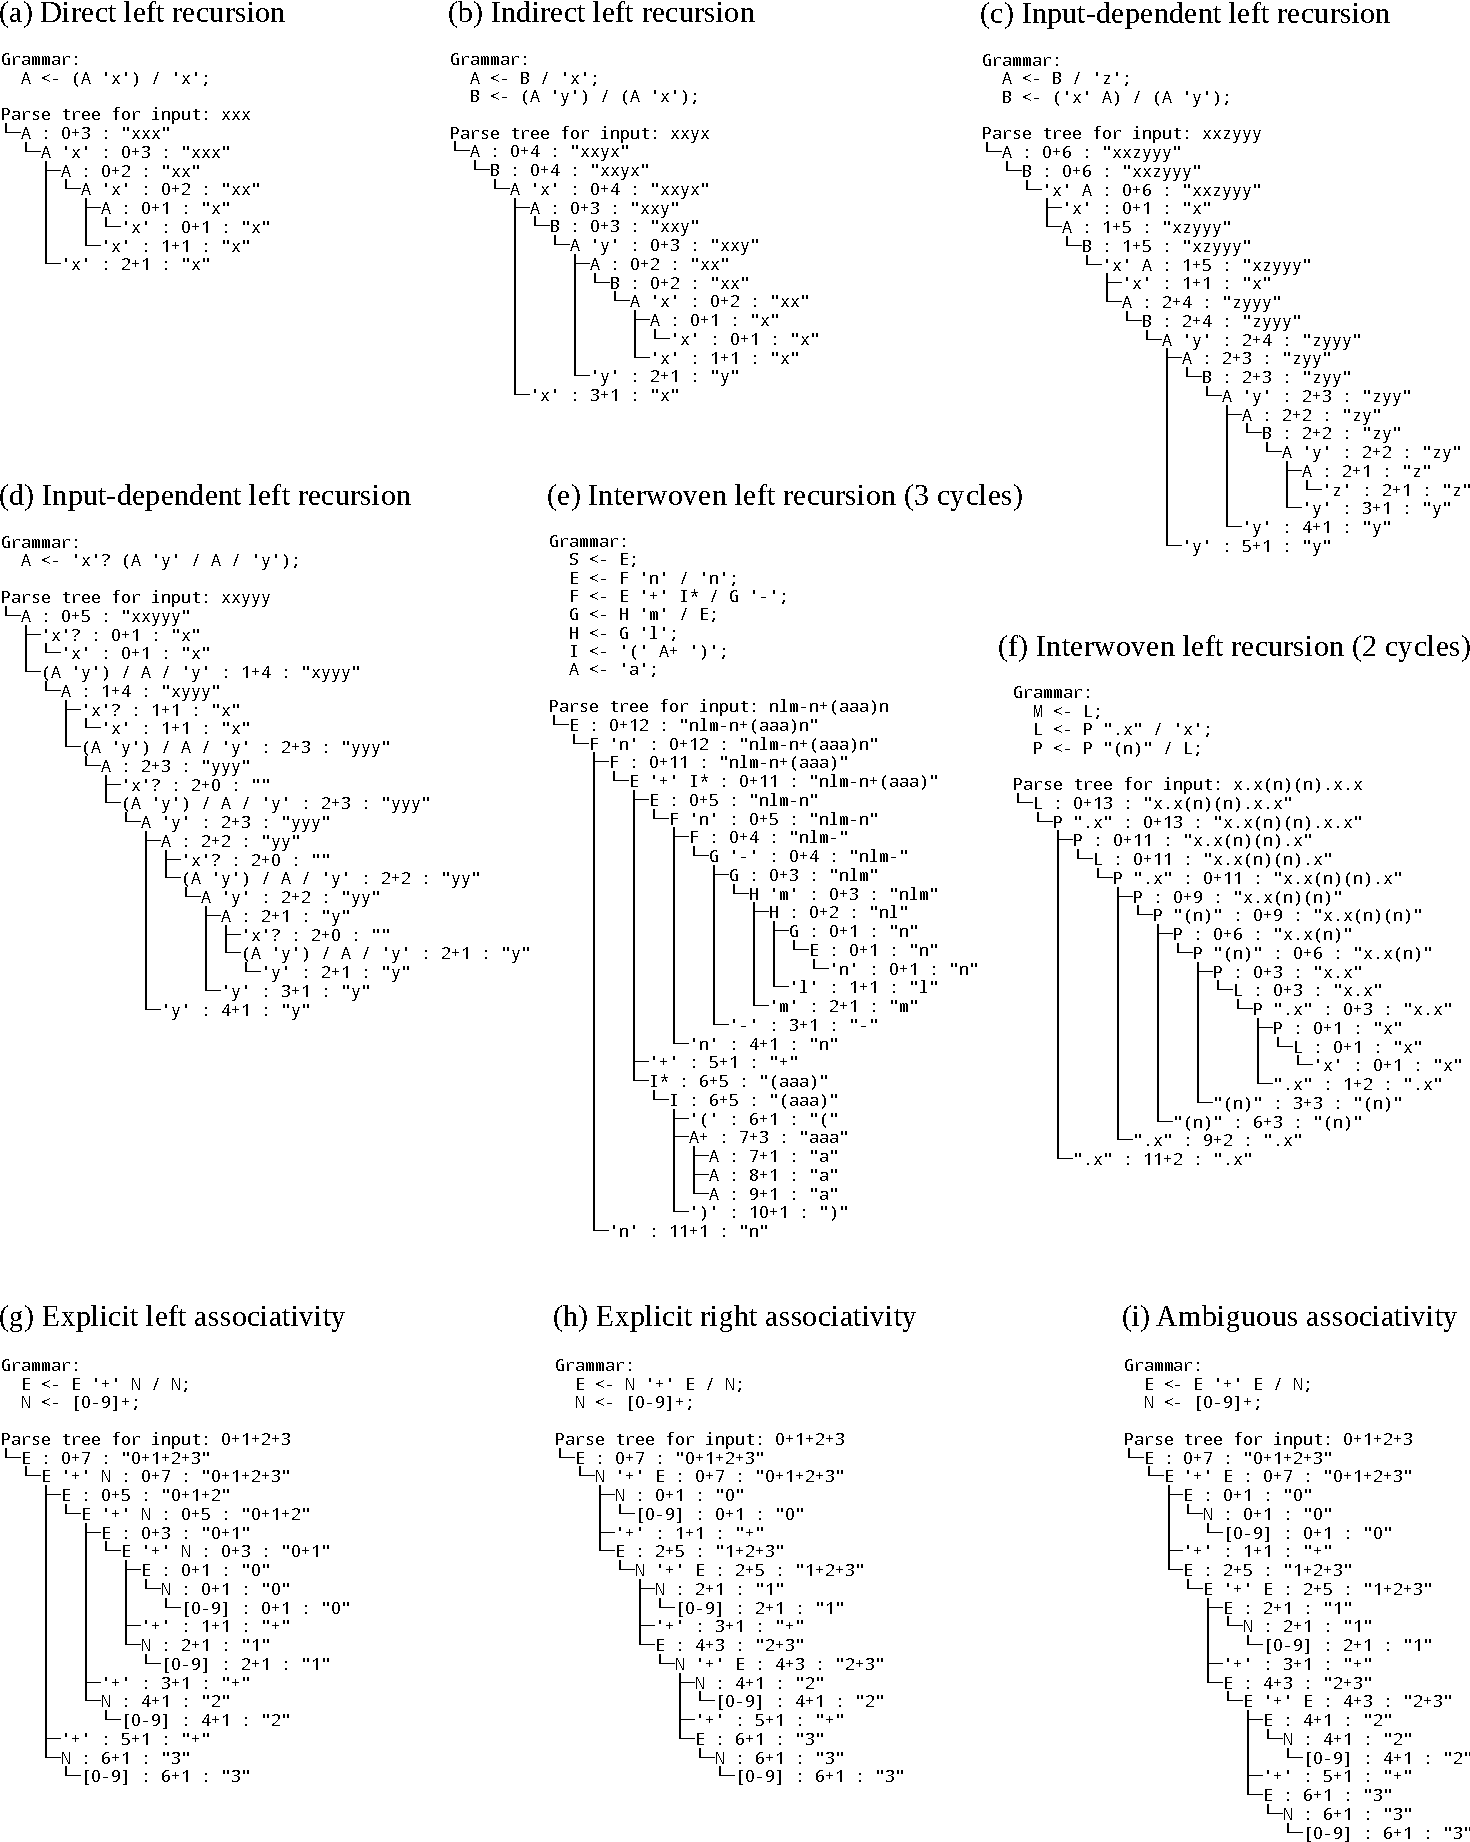
\includegraphics[width=0.98\textwidth]{Figs/LeftRecTypes.pdf}
\caption{\label{fig:LeftRecTypes}The parse tree created by the squirrel parser for a range of different left recursion types and associativity.}
\end{figure}

\section{Performance}

\subsection{Time complexity}

Because the expansion of each loop around a left recursive cycle is required to consume at least one additional character of the input, the squirrel parser retains the linear performance of the standard packrat parser, even when handling left recursive cycles. A parse tree cannot be deeper than the length of the input except by a constant factor, and the number of nodes in the parse tree must be linearly proportional to the length of the input, whether or not left recursive cycles are present in the grammar. The number of recursion frames plus the number of iterative left recursion expansion cycles performed by the squirrel parser is a linear function of the number of parse tree nodes created, since up to one parse tree node (one match) is created per recursion frame or iteration. Therefore, the amount of work performed by the squirrel parser is a linear function of the length of the input, no matter how the grammar is structured.

\subsection{Benchmarks}

The squirrel parser reference implementation (Section~\ref{sec:software}) was benchmarked against the following parsers:

\begin{table}[h!]
\centering
\begin{tabular}{c c c c c c c} 
    \hline
    Parser & Version & Language & Grammar Type & Lexer & Parser Type & Left Recursion Support \\
    \hline
    ANTLR4~\cite{parr2014,antlr4} & 4.9.2 & Java & LL(*) & Y & Parser generator & Direct only \\
    Parboiled1~\cite{parboiled1} & 1.3.1 & Java & PEG & N & Parser & None \\
    Parboiled2~\cite{parboiled2} & 2.3.0 & Scala & PEG & N & Macro/Combinator & None \\
    Mouse~\cite{mouse} & 2.3 & Java & PEG & N & Grammar-rewriting parser & Partial \\
    \hline
\end{tabular}
\caption{Benchmarked Parsing algorithms}
\label{table:1}
\end{table}

% Add section on optimizations: dense vs. sparse; collecting terminal trees to save memory and time

% JSON:
% Squirrel optimizations: collected String and number clauses into a single terminal matcher; used 2D memo table
% Large JSON documents (average size: 3.56MB; count: 100) -- Squirrel memoizes and Antlr does not (neither memoization nor backtracking is required for JSON parsing, which makes JSON a perfect usecase for ANTLR4, which rewrites the grammar into a form that requires neither of these -- this is most efficient for cases that can easily be parsed efficiently and directly by a recursive descent parser without memoization and backtracking, and can degrade to O(N^4) in the worst case if not).
% Squirrel: 15.52MB/sec (0.69x)
% Antlr4: 22.59MB/sec (1.00x)
% Small JSON documents (average size: 34B; count: 1000)  -- Squirrel has very low startup time, so has much better throughput than Antlr
% Squirrel: 11.37MB/sec (1.00x)
% Antlr4: 2.84MB/sec (0.25x)
%
% For comparison, https://github.com/GoogleChromeLabs/json-parse-benchmark :
% v8 version 8.4.371 : 0.554MB/sec calling JSON.parse on (a different) 8.2MB JSON string literal (14.808 sec)
% 6.99mb JSON file (quotes not escaped): Squirrel: 19.38MB/sec (0.361 sec); Antlr4:	20.43MB/sec (0.342 sec).


% Mouse Java 14 grammar: http://mousepeg.sourceforge.net/Grammars/Java.14.peg


% Expression parsing: 
% Squirrel optimizations: collected number clauses into a single terminal matcher; used 2D memo table
% maxDepth = 10; totLen = 37451 (for 40 inputs tot)
% Squirrel              SqrlLeftRec Mouse       MouseLeftRec        Antlr4      Parb1       Parb2
% 0.008453717000000001	0.013403438	4.546160006	4.3350593680000005	0.489739827	3.255461266	64.1386069
% Squirrel takes 2x as long with a left recursive grammar as expected, because each term could be left recursive and so has to be matched twice.
% Mouse is actually a little faster with a left rec grammar, presumably because the dual grammar is more efficient somehow.
% Mouse (both grammars) and Parboiled1 exhibit quadratic performance in the length of the input, and Parboiled2 exhibited cubic performance in the length of the input, so these were not included in a larger test.
% maxDepth = 18; totLen = 2602337 (for 40 inputs tot)
%   Squirrel non-left-rec grammar: 0.23281
%   Squirrel left-rec-grammar: 0.46838
%   Antlr: 43.15888


% Java parsing:
% Squirrel optimizations: collected whitespace, strings, identifiers, and number clauses into a single terminal matcher; used 2D memo table
% 4009 files, 8472606 bytes
% Parb1	Antlr/java	Antlr/java8	Antlr/java9	Mouse/java14	Squirrel/Parb1J6	Squirrel/MouseJ8	Squirrel/MouseJ14
% 4.812776823	1.900049109	146.910593906	197.78326554100002	94.06347794000001	1.154940077	1.732624619	2.7560864950000004
% Effect of using sparse memo table:
% 	Squirrel/Parb1J6	Squirrel/MouseJ8	Squirrel/MouseJ14
% Dense:	1.154940077	1.732624619 2.756086495
% Sparse:	1.064345105	2.216801828	12.629940091


% \begin{enumerate}
%     \item ANTLR4 version 4.9.2~\cite{parr2014,antlr4}. This is not a PEG parser, but rather an LL(*) parser generator. ANTLR is considered flexible and highly performant, as long as a grammar has been optimized for the parser. ANTLR4 can handle direct left recursion, but not indirect left recursion (ANTLR3 and earlier could handle neither). ANTLR compiles a lexer and parser, given tokenization rules and a grammar, which is part of its performance advantage, since the lexer and parser are custom-optimized for the grammar. Lexing or tokenization is also considered to increase performance, even though lexing can change the recognized language, since it is mostly a context-free process.
    
%     \item Parboiled version 1.3.1~\cite{parboiled1}. This is a PEG parser written in Java. Parboiled 1.x directly parses the input using the grammar, rather than compiling a custom parser.
    
%     \item Parboiled2 version 2.3.0~\cite{parboiled2}. This is a PEG parser generator written in Scala, so it compiles a custom parser for the grammar. Parboiled which does not support left recursion at all, in either version 1 or version 2.
% \end{enumerate}

%TODO: Java parsers: https://tomassetti.me/parsing-in-java/
% Optimized fork of Antlr: https://github.com/tunnelvisionlabs/antlr4/blob/master/doc/optimized-fork.md
% TODO: read and cite this paper: https://dl.acm.org/doi/10.1145/2814251.2814265 -- their parser is Autumn: https://github.com/norswap/autumn
% TODO: benchmark the Rats! parser, part of xtc: https://cs.nyu.edu/~rgrimm/xtc/
% TODO: include a JSON parsing benchmark -- Autumn and Parboiled2 contain JSON parsing code already, and probably ANTLR does too

% C++ parser than supports left recursion: https://github.com/axilmar/parserlib
% The Pegged PEG parser in D that supports all forms of left recursion -- see this for a great discussion of left recursion: https://github.com/PhilippeSigaud/Pegged/wiki/Left-Recursion

% A description of Medeiros' algorithm: https://github.com/pegjs/pegjs/issues/231#issuecomment-54756322

%TODO: go through comments in source code while writing up description of code

%TODO: mention that when OneOrMore / ZeroOrMore is implemented, it must stop if a zero-length sequence is matched.
%TODO: algorithm appears optimal or close to optimal, since there is little to no wasted or duplicated work. -- put in abstract?

%TODO: suggest Longest given the memo length increase heuristic. It also gives capability somewhere between First (ordered choice) and context free grammars, in that the order of subclauses is not important (except to break ties).
% Actually: the prefix problem (when First subclauses are in the wrong order) exactly shows why Longest is useful: if a prefix match prevents a longer match when the prefix is in an earlier subclause position, using Longest would eliminate this problem. First ordering is never a problem when one subclause cannot match a prefix of another subclause, and it's only a problem when it can't be determined which subclause can match a prefix of another subclause.

% TODO: Give an example of where greedy expansion of left recursion can result in failures:
% TODO: this example can't parse the input: T <- '-'? T '+' N / N; N <- [0-9]+; input="-1+2+3"
% TODO: the reason is that T will match "1+2+3", then T will try to match "-(1+2+3)+N", which fails.
% Better example: A <- 'x'? (A 'y' / A / 'y');  -- matches zero or more 'x's followed by one or more 'y's.
% If you try A <- 'x'? (A 'y' / 'y'); , it will fail if there are more 'x's than 'y's, and will skip any more 'y's than there are 'x's, but only if there is at least one 'x'.

% Re. Longest: ordering bugs in PEG grammars are a royal pain to deal with (they are by far the most annoying part of working with PEG grammars), and it is extremely difficult to debug these issues for large grammars, even with parsing visualization tools -- so it's better to use Longest in all cases *except* when you need a prefix to override a longer match. In other words, pick First to greedily choose prefixes over longer matches; choose Longest to greedily choose longer matches over prefixes.
%The only rule that actually backtracks is `First`, and that has a hard fast definition, which induces its semantics. The `Longest` rule I proposed effectively allows "backtracking across all possibilities", since all its subclauses are tested. The one that "wins" is the longest clause (with the earliest clause chosen if tiebreaking is needed). This comes closest to the "unlimited backtracking" that you are hinting with. And yes, it works with memoization / packrat parsing.
% Longest matches human intuition because for a wide range of human-readable languages, humans are able to pattern-match in a context-free way: any programmer can scroll into the middle of a program's source code and visually identify method definitions, variable assignments, expressions, case statements etc. -- we intuitively match the grammar rule that matches as much of the input as possible.

% Another good justification for Longer / PEG+:
% https://jeffreykegler.github.io/personal/timeline_v3 :
% PEG achieves unambiguity by finding only a subset of the parses of its BNF grammar. And, like its predecessor GTDPL, in practice it is usually impossible to determine what the subset is. The best a programmer usually can do is to create a test suite and fiddle with the PEG description until it passes. Problems not covered by the test suite will be encountered at runtime.
%
% PEG takes the old joke that the code is the documentation one step further -- with PEG it is often the case that nothing documents the grammar, not even the code. Under this circumstance, creating reliable software is impossible. As it is usually used, PEG is the nitroglycerin of LL parsing -- slightly more powerful than LL(1), but too dangerous to be worth it.


% ------------------------------------------------------------------------

%TODO: everything below here is old

% \section{A deep dive into the theory of left recursion}


% One of the reasons why a simple algorithm has not been previously found for parsing in the presence of left recursion may be that there are several misconceptions about left recursion and recursive descent parsing that have obscured the semantics of left recursion. These misconceptions are covered below, along with lemmas about how to properly handle left recursion that arise from correcting these misconceptions.

% \subsection{\label{sec:postorder}Misconception 1: recursive descent parsers produce the parse tree top-down}

% Because recursive descent parsers recurse down the grammar from the ``top rule'' towards the terminals, in order to build the parse tree for a given input, they are considered to be top-down parsing algorithms, in contrast to many parsing algorithms that work bottom-up. %TODO: refs
% However, a recursive descent parser does not build a parse tree node to correspond to the current recursion frame \emph{until all the required descendant clauses in the grammar have been found to match the input}. Restated, a recursive descent parser is a \emph{postorder} traversal (not a preorder traversal) of the grammar with respect to the input. (A clause in the grammar is only found to match the input if all its requisite subclauses match.)

% A postorder traversal actually builds the parse tree \emph{on the way back up}, right before the return from each recursion frame. Hence, \emph{even so-called top-down parsing algorithms would be more correctly thought of as bottom-up parsing algorithms}.

% \begin{lemma}
% Both top-down and bottom-up parsers build the parse tree bottom-up. Therefore, left-recursive grammar cycles should also be expanded into a parse tree in bottom-up order.
% \end{lemma}

% \subsection{Misconception 2: there is a difference between direct and indirect left recursion}

% Many previous papers have referred to ``indirect left recursion'' (where a rule doesn't refer directly to itself in a left-recursive way, but rather there is a path of rule references that lead back to the original rule, creating a left-recursive cycle). These papers often refer to indirect left recursion as being more difficult to parse than left recursion, %TODO: ref
% and indeed, the algorithms in these papers often don't handle indirect left recursion, because they just add in a special-case heuristic for rules directly referring to themselves in the leftmost subclause position. However, from a theoretical point of view, it makes no difference whether the path from a grammar rule back to itself has a length of one (``direct left recursion'') or more than one (``indirect left recursion'') -- all that matters in the classification of a path through the grammar as left recursive or non-left-recursive is whether or not at least one character is consumed while traversing each loop around each cycle in the path.

% \begin{lemma}
% There is no graph-theoretical difference between direct and indirect left recursion. Therefore, the expansion of a left-recursive cycle should be triggered the same way, no matter the path length of the cycle.
% \end{lemma}

% \subsection{\label{sec:monotonic}Misconception 3: grammar rules are either left recursive or right recursive}

% A grammar rule of the form \texttt{(E0 <- E0 '+' E1)} is often referred to as ``left recursive'' and a grammar rule of the form \texttt{(E0 <- E1 '+' E0)} is often referred to as ``right recursive''. However, there is really no such thing as right recursion, only left recursion and \emph{non-left recursion}\footnote{Although there is no such thing as a ``right-recursive grammar rule'', it is certainly possible to construct binary grammar rules that are left associative or right associative, producing a parse tree with the same associative structure. But even these cases are not as directly tied to left recursion and non-left recursion as it may seem. %TODO: link to section on how ambiguous grammars are right-associative by default.
% }. The distinction between the two is not whether the left operand or the right operand of a two-argument grammar rule is involved in a cycle, but \emph{whether or not the parser must monotonically advance, by matching at least one character of the input, before looping around a cycle in the grammar}. Paths through the grammar that consume zero characters before returning to the same grammar clause are left recursive; paths through the grammar that must consume at least one character before returning to the same grammar clause are not left recursive.

% The reason why a cycle in the grammar must consume at least one character for the cycle to be non-left-recursive is that if at least one character is consumed per loop around the cycle, then the cycle makes \emph{monotonic progress} in parsing the input. More technically, the only ``state'' visible to a recursion frame in a recursive descent parser (if we ignore the memo table) is the current location \texttt{(rule, pos)} of the parser: the current rule that is being matched against the input, and the start position within the input at which that rule is being matched. If such a state is revisited a second time in the same recursion path (i.e. if the current recursion path contains the same \texttt{(rule, pos)} pair at least twice), then by definition zero characters must have been consumed between the first occurrence and the second occurrence of that state (because \texttt{pos} is the same both times). Therefore, this state will repeat infinitely, meaning that the parser will get stuck in infinite recursion.

% Incidentally, this requirement for left recursive cycles in the grammar to consume at least one character, in order to ensure monotonic progress of the parser, is directly related to the reason why packrat parsers claim linear performance with respect to the length of the input: the parse tree can be no deeper than the length of the input, and the number of nodes in the parse tree cannot be greater than a constant multiple of the length of the input.

% \begin{lemma}
% The expansion of a left-recursive grammar cycle into a parse tree should require at least one character to be consumed per loop around the cycle, in order to ensure monotonic progress of the expansion process towards completion.
% \end{lemma}

% \subsection{Misconception 4: grammar rules are always either left recursive or not left recursive}

% To refine the previous claim, whether or not a path through the grammar causes a recursive descent parser to enter a left recursive cycle may depend upon the input parsed -- hence it is more accurate to think of a grammar rule as being either \emph{potentially left recursive, depending on the input}, or not left recursive.

% In Fig.~\ref{fig:LeftRecDependsOnInput}, the grammar causes a recursive descent parser to enter a left-recursive cycle for Input~2 but not for Input~1. Similarly, the grammar rule \texttt{(E <- B? C* E)} causes the parser to enter a left recursive cycle when \texttt{B} and \texttt{C} do not match the input (since both \texttt{(B?)} and \texttt{(C*)} will each match zero characters even if \texttt{B} and \texttt{C} do not match the input). This will cause the parser to fail to advance monotonically before again trying to match \texttt{E} in the same position.

% \begin{figure}
% \centering
% \begin{lstlisting}[frame=none,xleftmargin=.35\textwidth]
% Grammar:
%     A <- ('x' A) / 'y' / (A 'x');

% Input 1:            Input 2:
%     xxxy                yxxx
% \end{lstlisting}
% \caption{Grammar rule that may or may not cause a recursive descent parser to enter a left-recursive cycle, depending on the input.}
% \label{fig:LeftRecDependsOnInput}
% \end{figure}

% \begin{lemma}
% The process of expansion of left-recursive cycles in the grammar should not be triggered unless a left-recursive cycle is actually encountered (i.e. the decision about when to attempt expansion of left recursion is a property of a specific path through the grammar, given the input, and should not be triggered in response to the structure of the grammar itself).
% \end{lemma}

% \subsection{Misconception 5: packrat parsers always take time linearly proportional to the length of the input}

% One of the great accomplishments of the packrat parser is the claim that this algorithm takes time linearly proportional to the length of the input. %TODO: ref
% However, it is possible to construct pathological grammars that trigger an infinite loop in a na\"ive implementation of a packrat parser. Thus in the worst case, technically a packrat parser scales not as $O(N)$, but rather $O(\infty)$, i.e. does not terminate. The reason for this is again related to the distinction between left recursion and non-left recursion, i.e. whether or not monotonic progress is made towards the end of the input while recursing or iterating.

% The simplest grammar that can cause a na\"ive packrat parser to enter an infinite loop is $\epsilon*$, i.e. ``match the empty string zero or more times''. The empty string terminal $\epsilon$ matches zero characters, then the \texttt{ZeroOrMore} operator will continue to consume this zero-length match until it no longer matches -- however the empty string will always match, and the parser will not advance, leading the \texttt{ZeroOrMore} to match an infinite number of times (or rather, up to RAM limits, since a node will be added to the parse tree for each zero-length match).

% In practice, this degradation to an infinite loop can be prevented by never allowing \texttt{ZeroOrMore} or \texttt{OneOrMore} clauses to consume more than one zero-length subclause match; however, the parser must be written defensively, with this protection against pathological grammars (and grammars that may exhibit this behavior given certain pathological inputs) in mind.

% Every iterative algorithm has a recursive equivalent. A close recursive analog of iteratively matching $\epsilon*$ is left recursion: with left recursion, a standard recursive descent parser makes no forward progress through the input at each recursion frame, so ends up recursing infinitely (at least until the stack is full). Memoization does not prevent this, because a match is memoized only \emph{on exit} from recursion (because recursive descent parsing is a postorder traversal of the grammar with respect to the input). These recursion frames will never exit -- the parser only continues to recurse deeper as it loops around a grammar cycle. As with $\epsilon*$, where the simple fix was to allow only one iterative match if the match has length zero, for left recursion, the simple fix is to allow only one recursion through a left-recursive cycle (since this consumes zero characters), by keeping a set of \texttt{(clause, pos)} parse states, and stopping recursion as soon as the same parse state is visited twice.

% However, simply terminating recursion when a cycle is encountered does not allow the left recursion to be ``unrolled'' to usefully match the input. Instead, the point at which a left-recursive cycle is ``completed'' is the point at which expansion of the cycle may begin.

% \begin{lemma}
% The process of expansion of left-recursive cycles in the grammar should be triggered once the same grammar rule is visited at the same input position twice in the same recursion path.
% \end{lemma}

% \subsection{\label{sec:Omniscient}Misconception 6: There is no reasonable way to interpret left recursion}

% It may appear that there is no reasonable way to interpret a left-recursive grammar cycle in a recursive descent context, other than as an infinite loop, based on how recursion is defined. However, if we require that every loop around any cycle in the grammar (whether left recursive or not) consume at least one character, then no cycle will ever lead to infinite recursion, including (if handled correctly) a left-recursive cycle. The job of the left-recursion-capable parser is then to figure out exactly how many characters should be consumed by each rule in a left-recursive cycle, while ensuring at least one character is consumed by at least one rule for each loop around the cycle, regardless of the path length of the cycle.

% Given a complete and correct parse tree (the output of a correct parse), the input string that the parse tree was produced from, and a grammar, it is possible to check in linear time whether the parse tree matches the input, given the grammar (even if the grammar contains left-recursive cycles).

% Similarly, we may consider an \emph{omniscient parser} that works ``backwards'' (relative to a recursive descent parser), where the correct structure of the next set of branches in the parse tree can be divined correctly \emph{a priori} by the omniscient parser at all points while it is recursively constructing the data structure of the parse tree. An omniscient parser doesn't need to complete the process of recursion to all subclauses before it is able to match the current clause, producing a parse tree node. In other words, an omniscient parser represents a \emph{preorder} traversal of the grammar with respect to the input, as opposed to the postorder traversal employed by standard recursive descent parsing -- and thus an omniscient parser builds the parse tree top-down, not bottom-up (Section~\ref{sec:postorder}). An omniscient parser can also be thought of as a nondeterministic parser, which considers all possible match lengths of all subclauses of each clause in parallel, and discards any parses that don't fit the input, producing only correct parse trees. If there is more than one correct parse tree for the whole input, then a heuristic (which matches the semantics of the grammar rules) can be used to select a single final parse tree.

% An omniscient parser, presented with a left-recursive grammar cycle, is able to discern \emph{a priori} how many loops around a grammar cycle will match the input, and will build the corresponding subtree of the parse tree to exactly that height.

% Note that even an omniscient parser is bound by the requirement that each loop around a left recursive grammar cycle must consume at least one character, so that monotonic progress is made with each successively deeper loop around the cycle, so that the parser doesn't enter the same state more than once, causing it to recurse infinitely (Section~\ref{sec:monotonic}). Because the length of the input is finite, and because at least once character of the input must be consumed by each loop around a left recursive grammar cycle, the parse tree must be of finite height, meaning that eventually a clause in the cycle must fail to match, terminating recursion. 

% Call this lowest failed match attempt the \emph{fixed point} of the cycle. The termination of the cycle at this fixed point will fail over to other rules outside the left-recursive cycle, or to terminal clauses in the grammar, yielding leaves in the parse tree.

% \begin{lemma}
% If we ensure that every loop around a left-recursive cycle consumes at least one character, then because the input is finite, recursive descent through a left-recursive cycle must eventually terminate with some rule in the cycle failing to match the input. Expansion of the left-recursive cycle will build the parse tree upwards from this \emph{fixed point}.
% \end{lemma}

% \subsection{Misconception 7: Handling left recursion must degrade parser performance to superlinear}

% Since it is impossible to implement an omniscient parser using a deterministic Turing machine. A non-omniscient recursive descent parser cannot know \emph{a priori} exactly how many loops around each left-recursive cycle to descend at each input position. However, if the recursion depth were in fact known \emph{a priori}, then the parser could be modified to accept a ``recursion depth counter'' that was set to the known recursion depth at the beginning of left recursion. This counter would then be decremented for each loop around the left recursive cycle. Once the counter reached zero, the left-recursive clause would be marked as a mismatch, forming the fixed point of the cycle, and returning from its recursion frame. The standard recursive descent algorithm would then correctly build the parse tree on exit from each successively higher recursion frame. Medeiros et al. termed this recursion to a fixed depth ``bounded left recursion''. %TODO: ref

% However, for non-omniscient recursive descent parsing, this recursion depth cannot be known \emph{a priori} for a left recursive grammar rule at any specific position within the input. Instead, when an attempt is made to match a left-recursive grammar rule, we could attempt bounded left recursion to successively greater depths, by starting with a depth bound of 1, and then successively increasing the depth bound by 1, until some stopping criterion was reached. Warth et. al. termed this ``growing the seed''. %TODO: ref

% Without memoization, this method of successively increasing the depth bound until the grammar cycle no longer matches would exhibit quadratic performance at best (or exponential at worst). With memoization, the parse subtree found with the previous depth bound can be incorporated directly from the memo table as a subtree, without repeating the work. This reduces the amount of work that needs to be done when expanding the left-recursive cycle, to linear in the length of the input.

% \begin{lemma}
% If the process of expansion of a left-recursive cycle relies on memoization, the resulting parser will still take time linear in the length of the input.
% \end{lemma}

% \subsection{\label{sec:StoppingCriterion}Misconception 8: It is sufficient to stop expanding left recursion when match length stops increasing}

% Since a completed parse tree only includes matches of grammar rules to the input, and not mismatches, and since we require that each loop around a left-recursive cycle consumes at least one character, the most intuitive stopping criterion for the expansion of a left-recursive cycle is the point at which the match length does not increase for a clause in the cycle. The most recent match (not including the final mismatch) then becomes the match for the entire grammar cycle, and the left recursion expansion process terminates.

% In a memoizing parser, this stopping criterion can then be implemented by ensuring that a match in the memo table is never replaced by a mismatch, and that and older match is only replaced by a newer match if the newer match consumes at least one character more of the input than the older match. Then left recursion expansion will continue until the memo table for the clause and position remains unchanged after trying to expand the left-recursive cycle.

% This stopping criterion has been used previously for expanding left-recursive matches. %TODO: ref -- Medeiros, and also Warth? (growing the seed).
% However, the validity of this criterion has not been examined closely in previous work. In fact, it is possible to construct grammars that show that this stopping criterion is insufficient to parse some inputs, given some grammars.

% For the grammar and input given in Fig.~\ref{fig:Fail1}, an omniscient parser will match the entire input, \texttt{xxyx}. However, for a non-omniscient recursive descent parser, the process of expansion of left recursion will only match the first three characters of the input, \texttt{xxy}, if the parser memoizes \emph{individual clauses} of the grammar (\texttt{(B !'y')}, \texttt{(!'y')}, \texttt{'y'}, \texttt{'x'}, \texttt{(A 'x')}, and \texttt{'x'}), rather than at the coarser granularity of rules (\texttt{A} and \texttt{B}).

% \begin{figure}
% \centering
% \begin{lstlisting}[frame=none,xleftmargin=.35\textwidth]
% Grammar:
%     A <- B / 'x';
%     B <- (A 'y') / (A 'x');

% Input:
%     xxyx
% \end{lstlisting}
% \caption{Example grammar where stopping the expansion of left recursion once a longer match cannot be found may fail to match the input, depending on how matches are memoized.}
% \label{fig:Fail1}
% \end{figure}

% \begin{figure}
% \centering
% \begin{lstlisting}[frame=none,xleftmargin=.35\textwidth]
% Grammar:
%     A <- (B !'y') / 'x';
%     B <- A 'x';

% Input:
%     xxxy
% \end{lstlisting}
% \caption{Example grammar where stopping the expansion of left recursion once a longer match cannot be found will fail to match the input unless a special exception is made for \texttt{First} clauses at the end of the expansion process.}
% \label{fig:Fail2}
% \end{figure}



% \begin{lemma}
% % TODO
% \end{lemma}

% \subsection{\label{sec:MemoizeRule}Effect of granularity of memoization on left-recursive parsing behavior}


% We can at least observe that both non-left recursion and expansion of a left recursive cycle involves greedily matching the grammar to the input, recursing as deeply as possible as the ``primary axis'' of movement, and then only proceeding to match any siblings of clauses in the left recursive cycle as the ``secondary axis'' of movement, bottom up, before exiting each recursion frame. However, does the stopping criterion for expansion of left-recursive cycles match the behavior of the omniscient parser, or more concretely, does the stopping criterion for expansion of left-recursive cycles produce behavior analogous to the behavior of a standard recursive descent parser working with non-left-recursive cycles?

% In Fig.~\ref{fig:LeftRecSemanticDiff_a}, the omniscient parser would match only a single character of the input, \texttt{x}. The reason is that the first subclause of \texttt{A}, \texttt{(B !'y')}, will greedily consume as many \texttt{x} characters as possible via the left-recursive cycle, until no more \texttt{x} characters can be consumed. The next character \texttt{y} will cause \texttt{(B !'y')} to fail to match, therefore rule \texttt{A} fails over to the final \texttt{'x'} subclause. This second subclause is matched starting again from the beginning of input (since the first subclause of \texttt{A} failed to match). The result therefore matches only the first \texttt{x} character in the input, leaving the remaining \texttt{xxy} unmatched.

% % \begin{figure}
% % \centering
% % \begin{subfigure}[t]{.4\linewidth}
% % \begin{lstlisting}[frame=none,xleftmargin=.2\textwidth]
% % Grammar:
% %     A <- (B !'y') / 'x';
% %     B <- A 'x';

% % Input:
% %     xxxy
% % \end{lstlisting}
% % \caption{\label{fig:LeftRecSemanticDiff_a}}
% % \end{subfigure}
% % \hspace{5mm}
% % \begin{subfigure}[t]{.4\linewidth}
% % \begin{lstlisting}[frame=none,xleftmargin=.2\textwidth]
% % Grammar:
% %     A <- B / 'x';
% %     B <- (A 'y') / (A 'x');

% % Input:
% %     xxyx
% % \end{lstlisting}
% % \caption{\label{fig:LeftRecSemanticDiff_b}}
% % \end{subfigure}
% % \caption{Examples of grammars where the proposed stopping criterion for expansion of left recursion by a recursive descent parser (Section~\ref{sec:StoppingCriterion}) may fail to match the input in the same way as an omniscient parser (Section~\ref{sec:Omniscient}), depending on how matches are memoized (Section~\ref{sec:MemoizeRule}).}
% % \label{fig:LeftRecSemanticDiff}
% % \end{figure}

% In contrast, in a non-omniscient parser, iteratively expanding the left-recursive cycle until the stopping criterion is triggered will cause the parser to match the first two characters of the input, \texttt{xx}, rather than only the first character, \texttt{x}, but \emph{only if individual grammar clauses are separately memoized, rather than rules}. If the \texttt{(B !'y')} subclause of \texttt{A} is memoized each time it is matched, then given the condition that a memo table entry may never be downgraded from a match to a mismatch (Section~\ref{sec:StoppingCriterion}), \texttt{(B !'y')} will never be memoized as a mismatch, so rule \texttt{A} will never fail over from the first subclause to the second subclause. Therefore, a left-recursion-capable recursive descent parser will end up matching the first two characters of the input, \texttt{xx}, and then stop matching, instead of failing over like the omniscient parser to match just the first character of the input, \texttt{x}. If instead the memo table contains entries only at the level of granularity of rules (here \texttt{A} and \texttt{B}), and not for individual clauses (here \texttt{(B !'y')}, \texttt{(!'y')}, \texttt{'y'}, \texttt{'x'}, \texttt{(A 'x')}, and \texttt{'x'}), then the proposed stopping criterion produces the same behavior in a left-recursion-capable recursive descent parser as it does in the omniscient parser.

% Fig.~\ref{fig:LeftRecSemanticDiff_b} exhibits a similar difference in behavior between the two types of parser. For this example, the omniscient parser will match the whole input, \texttt{xxyx}, whereas iterative expansion of the left-recursive cycle from the fixed point will match only \texttt{xxy} if individual subclauses are memoized, as opposed to whole rules. In this case, the reason for the failure of the left-recursion-capable recursive descent parser to match the whole input is that the memo entry for the first subclause of \texttt{B}, i.e. \texttt{(A 'y')}, will never be downgraded in the memo table from matching \texttt{xxy} to failing to match \texttt{xxyx}, and without this mismatch, rule \texttt{B} cannot fail over to the second subclause, \texttt{(A 'x')}, in order to match the full input. If \texttt{B} does not match the full input, then the top rule \texttt{A} is also unable to match the whole input.

% The solution to this difference in behavior (at least for these two examples) is for the left-recursion-capable recursive descent parser to memoize at the granularity of rules, rather than at the level of individual clauses within the tree of clauses of a rule. However, it is worth hypothesizing that even with this adjustment, there may be other cases of larger-scale behavioral differences between the omniscient parser and a memoizing left-recursion-capable recursive descent parser -- although examples of this are not known at this time. We will proceed under the assumption that larger-scale examples of disparity in behavior do not exist; however, whether or not such examples exist is left as an open question for further research.

% \subsection{\label{sec:WeirdFirst}The curious case of \texttt{First}}

% A parser can parse left recursive grammar cycles as long as each loop around the cycle consumes at least one additional character, ensuring that the parser always makes monotonic progress (Section~\ref{sec:monotonic}). However, if a left-recursive cycle contains a \texttt{First} clause, it is conceivable that the match length will \emph{decrease} in length between two successive expansions of the cycle. In fact we see this behavior with Fig.~\ref{fig:LeftRecSemanticDiff_a}: the omniscient parser first matches \texttt{x}, then \texttt{xx}, then fails to match \texttt{xxx} (because it is followed by \texttt{y}), then rule \texttt{A} fails over to the second subclause of the \texttt{First} clause, and the match length \texttt{A} decreases from 2 to 1 for the final match of \texttt{x}.

% We need to consider the behavior of \texttt{First} in the context of our requirement that matches consume at least one additional character per loop around a grammar cycle. Consider a \texttt{First} clause with at three subclauses, \texttt{C\textsubscript{0}}, \texttt{C\textsubscript{1}} and \texttt{C\textsubscript{2}}. In the previous stage of expansion of the left-recursive cycle, \texttt{C\textsubscript{0}} failed to match, and \texttt{C\textsubscript{1}} matched. In the current stage of expansion of the left-recursive cycle, 

% \subsection{\label{sec:LeftRecExpansionCriteria}Final criteria for valid expansion of left-recursive cycles}

% To summarize, the conditions under which left recursive cycles can be safely expanded (i.e. repeatedly matched against the grammar, bottom-up, until a stopping criterion is met), are:

% \begin{enumerate}
%     \item Memoization is applied at the granularity of rules (and not of clauses within rules).
%     \item The expansion of a left recursive cycle is seeded by writing a mismatch into the memo table for the clause that completed the cycle. (This is the fixed point of the cycle.)
%     \item Each successive match attempt must produce a longer match than the previous match attempt, otherwise the memo table should not be updated with the new match result: a match of zero or more characters replaces a mismatch in the memo table; a longer match replaces a shorter match. This ensures that the parser makes monotonic progress.
%     \item A mismatch should never replace a match in the memo table. This enables the stopping criterion.
%     \item Expansion of a left recursive cycle stops when the memo table entry is unchanged after the most recent match attempt. This enforces the stopping criterion, ensuring that expansion of a left recursive cycle stops once the match can no longer be improved.
% \end{enumerate}




% TODO: (referred to as ``growing the seed'' in \cite{TODO}). %TODO: add ref


\section{Automatic conversion of parse tree into an Abstract Syntax Tree (AST)}

% TODO

\section{Error Recovery}

Syntax error classification and recovery has proved difficult to add to recursive descent parsers, and is an area of active research. %TODO ref
The squirrel parsing algorithm as presented does not attempt to solve this problem. If a squirrel parser fails to match the whole input, the location of the first syntax error can generally be identified by searching the memo table for the largest position of any mismatch. Error recovery work will continue as future research.

\section{\label{sec:software}Reference implementation}

An MIT-licensed reference implementation of the squirrel parser is available at: \url{http://github.com/lukehutch/squirrelparser}

\section{Conclusion}

% TODO

\bibliographystyle{ACM-Reference-Format}
\bibliography{main}

\end{document}
\endinput


